\documentclass[english]{article}
\usepackage{amstext}
\usepackage{amssymb}
\usepackage[utf8]{inputenc}
\usepackage[T1]{fontenc}
\usepackage{babel}
\usepackage{amsmath}
\usepackage{graphicx}
\usepackage{caption}
\usepackage{multirow}
\usepackage{slashed}
\usepackage[normalem]{ulem}
\usepackage[usenames,dvipsnames]{color}
\usepackage{fancyhdr}
\pagestyle{fancy}
\fancyhf{}
\renewcommand{\headrulewidth}{0pt}
\setlength{\headheight}{40pt} 

\begin{document}

\title{Looking beyond the Standard Model: \\Neutrino oscillations - history and current status}
\author{Candidate Number: 6950X}
\date{Suprevised by Dr Tina Potter}
\maketitle

\thispagestyle{fancy}

\begin{abstract}
In this review, we will have a detailed look at the history of neutrinos in the Standard Model as well as why and how it is extended to account for phenomena related to neutrinos. Past and current experiments on this topic and their status will also be discussed.
\end{abstract}

\section{Neutrinos and the Standard Model}
	Pauli first proposed the existence of neutrinos ("neutrons") in 1930 \cite{pauliletter1930} when he was looking at the problem of radioactive $\beta$-decay, in which the emitted electrons had a continuous spectrum of energies leading to contradiction with the principle of energy conservation. Pauli suggested that there must be another unseen particle, of spin $1/2$ and mass of the same order of magnitude as the electron mass, emitted along with the electron in order for energy to be conserved.
    
    In 1934, Fermi used Pauli idea as the basis of his famous theory of $\beta$-decay and generally theory of weak interaction \cite{fermi1934}, coining the name "neutrino" ("little neutral one") in the process. Fermi was then able to calculate the probability of neutrino detection, which came out to be so small that it prompted Bethe and Peierls to claim that neutrinos might never be observed \cite{bethepeierls1934}. However, in 1956 Cowan and Reines succeeded in doing just that \cite{cowanreines1956} by their discovery of the antineutrinos in nuclear reactor using the inverse beta decay process
    \begin{gather}
    	\bar{\nu}+p \rightarrow n+e^{+}
    \end{gather}
    
    After parity was found not to be conserved in the $\beta$-decay and other weak processes \cite{wu1957} by Wu \textit{et al.} in 1957, Salam \cite{salam1956}, Landau \cite{landau1957}, Lee and Yang \cite{leeyang1957} put forward the theory of the two-component neutrino using Weyl previously rejected idea of two-component spinors \cite{weyl1929}. Consider the Dirac equation for the neutrino field with mass $m_{\nu}$
    \begin{gather}
    	i\gamma^{\alpha} \partial_{\alpha} \nu (x) - m_{\nu} \nu (x) = 0
    \end{gather}
    
    For left-handed (LH) and right-handed (RH) components, $\nu_{L} (x)$ and  $\nu_{R} (x)$, we obtain two coupled equations
    \begin{gather}
    	i\gamma^{\alpha} \partial_{\alpha} \nu_{L} (x) - m_{\nu} \nu_{R} (x) = 0 \\
        i\gamma^{\alpha} \partial_{\alpha} \nu_{R} (x) - m_{\nu} \nu_{L} (x) = 0
    \end{gather}
    
    Salam, Landau, Lee and Yang chose to assume that neutrino mass is zero, which is a reasonable assumption given the data existed at the time. If this is the case, we have two decoupled Weyl equations
    \begin{gather}
    	i\gamma^{\alpha} \partial_{\alpha} \nu_{L,R} (x) = 0
    \end{gather}
    and then the neutrino field can either be $\nu_{L} (x)$ or $\nu_{R} (x)$.
    
    The two-component theory implies the parity violation in $\beta$-decay and other weak processes (in agreement with the experimental results of the Wu \textit{et al.} and other experiments \cite{wu1957} \cite{garwinledermanweinrich1957}), and neutrino (antineutrino) helicity is equal to $-1$ ($+1$) if the field is $\nu_{L} (x)$ and is equal to $+1$ ($-1$) if the field is $\nu_{R} (x)$.
    
    In 1958, the helicity of neutrinos was measured from the chain reaction
    \begin{gather}
    	e^{-} + {}^{152} Eu \rightarrow {}^{152} Sm^{*} + \nu_{e} \\
        {}^{152} Sm^{*} \rightarrow {}^{152} Sm + \gamma
    \end{gather}
    by Goldhaber \textit{et al.} \cite{goldhabergrodzinssunyar1958}. The neutrino helicity was negative in full agreement with the two-component theory of massless neutrino, and it looks like from the two possibilities, $\nu_{L} (x)$ or $\nu_{R} (x)$, nature pick the first one.
    
    The two-component theory was built on the assumption that neutrinos have vanishing mass. This point of view was challenged after Feynman and Gell-Mann \cite{feynmangellmann1958}, Sudarshan and Marshak \cite{sudarshanmarshak1958} proposed their $V - A$ theory in 1958, suggesting that the violation of parity in the weak interaction is not connected with exceptional properties of neutrinos. Nevertheless, the two-component theory of massless neutrino was the simplest theoretical possibility and it still produced predictions that were consistent with the contemporary experiments on weak processes.
    
    In the following few years, the theory of electroweak interactions was formulated under the assumption of massless two-component neutrinos \cite{glashow1961} \cite{goldstonesalamweinberg1962} \cite{weinberg1967}. Together with the theory of the strong interaction \cite{grosswilczek1973} \cite{politzer1973}, the full theory describing all elementary particle interactions is known as the \textit{Standard Model} (SM).

\section{Neutrino Oscillations}
	The problems of the SM picture of neutrinos began with the Homestake experiment headed by Davis \cite{davis1968}. In 1968, Davis attempted to detect the solar neutrinos based upon the reaction
    \begin{gather}
    	\nu_{e} + {}^{37} Cl \rightarrow e^{-} + {}^{37} Ar
    \end{gather}
    A 380 cubic meter tank of a fluid rich in chlorine called perchloroethylene was placed 1,478 meters deep underground in the Homestake Gold Mine in South Dakota, USA to prevent interference from cosmic rays. Helium was bubbled through the fluid periodically to remove the argon that had formed, which were then counted by means of their radioactivity to determine how many neutrinos had been captured.
    
    Although solar neutrinos were successfully detected by Davis, a new problem emerged. The experimental results were consistently very close to one-third of Bahcall's calculations, that is the flux of neutrinos found by the detector was only one-third the amount theoretically predicted by the Standard Solar Model (SSM) \cite{davis1998} \cite{bahcall2004}. This discrepancy was known as the \textit{Solar Neutrino Problem}. Many physicists believed that the solution lies with a wrong neutrino flux given by the SSM or a mistake made by Davis while carrying out the experiment, but not with the SM. However, other subsequent experiments with the same purpose such as Kamiokande and later Super-Kamiokande in Japan e.g.\cite{kamiokande1991} \cite{superk2016}, SAGE in the former Soviet Union e.g.\cite{sage1991}, GALLEX in Italy e.g.\cite{gallex1999}, and SNO in Canada e.g.\cite{sno2001} confirmed the results of Davis.
    
    Similar alarming findings were found in the atmospheric neutrino flux, with several experimental groups observing a deficit in the number of atmospheric neutrinos produced by cosmic rays impacting on the Earth’s atmosphere e.g\cite{hirata1998} \cite{casper1991} \cite{macro1998}. This became the \textit{Atmospheric Neutrino Anomaly}.
    
    By the end of the nineties, it appeared likely that the SM has to be extended to explain these phenomena. The theory required, \textit{neutrino oscillations}, however, had been invented as long ago as 1957 by Pontecorvo \cite{pontecorvo1957}, who suggested that $\nu \Leftrightarrow \bar{\nu}$ transitions can occur in analogy with the $K^{0} \Leftrightarrow \bar{K}^{0}$ oscillation proposed earlier by Gell-Mann and Pais in 1955 \cite{gellmann1955}. Based on this idea, the theory of flavour neutrino mixing was first developed by Maki, Nakagawa, and Sakata in 1962 \cite{mns1962}, in which they assumed that the flavour eigenstates $\nu_{e}$ and $\nu_{\mu}$ ($\nu_{\tau}$ had yet to be discovered at the time) are not mass eigenstates, but are superposition of two "true neutrinos" with different masses
    \begin{gather}
    	\nu_{e} = \nu_{1} \cos\delta + \nu_{2} \sin\delta \\
        \nu_{\mu} = -\nu_{1} \sin\delta + \nu_{2} \cos\delta
    \end{gather}
    through some orthogonal transformation characterised by an angle $\delta$. The significance of this theory is that in order for mass to be a valid labeling scheme, it suggests that \textit{neutrinos must have finite mass}. This is different from the assumption of the two-component massless neutrino theory that the SM was previously built upon.
    
    The theory was further elaborated by Pontecorvo in 1967 \cite{pontecorvo1967}. In 1969, a year after the first solar neutrino deficit was observed in the previously mentioned Homestake experiment, Gribov and Pontecorvo followed up by publishing another paper \cite{pontecorvo1969}, in which they described quantitatively the idea of $\nu_{e} \Leftrightarrow \nu_{\mu}$ oscillations and how it might explain the decrease in the number of detectable solar neutrinos at the Earth surface. The first full version of the theory was worked out in several papers in the seventies \cite{fulltheory70s}. However, judging from the number of publications that are still emerging, this subject is still up for debate.
    
    All existing data on neutrino oscillations can be described within the
framework of 3-flavour neutrino mixing in vacuum. In its simplest form it can be expressed as a unitary transformation relating the flavour and mass eigenstates
	\begin{gather}
    	\nu_{lL} (x) = \sum_{j=1}^{3} U_{lj} \nu_{jL} (x)
    \end{gather}
    where $\nu_{lL} (x)$ is the LH flavour neutrino field $l=e,\mu,\tau$; $\nu_{jL} (x)$ is the LH component of the field of neutrino having definite mass $m_{j} \neq 0$, $j=1,2,3$; and $U_{lj}$ is the neutrino mixing matrix. The matrix $U$ is often called the Pontecorvo-Maki-Nakagawa-Sakata (PMNS) or sometimes simply Maki-Nakagawa-Sakata (MNS) mixing matrix.
    
    The mixing matrix $U$ is given by
    \begin{gather}
    	U =
        	\begin{bmatrix}
            	c_{12}c_{13} & s_{12}c_{13} & s_{13}e^{-i\delta}\\
                -s_{12}c_{23}-c_{12}s_{23}s_{13}e^{i\delta} & c_{12}c_{23}-s_{12}s_{23}s_{13}e^{i\delta} & s_{23}c_{13}\\
                s_{12}s_{23}-c_{12}c_{23}s_{13}e^{i\delta} & -c_{12}s_{23}-s_{12}c_{23}s_{13}e^{i\delta} & c_{23}c_{13}
            \end{bmatrix} .
            \begin{bmatrix}
            	1 & 0 & 0\\
                0 & e^{i\alpha_{21}/2} & 0\\
                0 & 0 & e^{i\alpha_{31}/2}
            \end{bmatrix}
    \end{gather}
    where $c_{ij}=\cos\theta_{ij}$, $s_{ij}=\sin\theta_{ij}$, the angles $\theta_{ij}=[0,\pi/2)$; $\delta=[0,2\pi]$ is the Dirac CP violation (CPV) phase; and $\alpha_{21}$, $\alpha_{31}$ are two Majorana CPV phases.
    
    The neutrino oscillation probabilities depend, in general, on the neutrino
energy $E$, the source-detector distance $L$, the elements of $U$, and the mass squared differences $\Delta{m_{ij}^{2}}=m_i^{2}-m_j^{2}$, $i \neq j$. In the 3-neutrino mixing framework, there are only two independent mass squared differences, say $\Delta{m_{21}^{2}} \neq 0$ and $\Delta{m_{31}^{2}} \neq 0$. The numbering system is arbitrary, although it proves convenient to identify $|\Delta{m_{21}^{2}}|$ with the smaller of the two neutrino mass squared differences. We also adapt the convention that $m_{1}<m_{2}$, so that $\Delta{m_{21}^{2}}>0$. The sign of $\Delta{m_{31}^{2}}$ is not yet determined. With these choices, if $\Delta{m_{31}^{2}}>0$ ($\Delta{m_{31}^{2}}<0$) the scheme is called normal (inverted) ordering NO (IO).

\section{Current Status}
	Most recent global neutrino fits within the standard 3-neutrino mixing framework can be found in \cite{esteban2017} \cite{capozzi2017} \cite{salas2018}. Here, the results of the most current fit \cite{salas2018} will be the main focus. Different past and present experiments contributing to the global neutrino analysis will be discussed, grouped in the accelerator, reactor, solar, and atmospheric sectors, followed by the results of the global analyses of neutrino oscillations data.

\subsection{Accelerator neutrino experiments}

	For experiments using accelerator neutrinos as the source, "long-baseline"
means that $E/L \simeq \Delta{m^{2}} \simeq 2.5 \times 10^{-3} eV^{2}$. The goals of the first long-baseline accelerator experiments proposed in the nineties, K2K \cite{k2k}, MINOS \cite{minos}, and CERN to Gran Sasso (CNGS) experiments OPERA \cite{opera} and ICARUS \cite{icarus} were to clarify the origin of the anomaly observed in the atmospheric neutrino measurements of Kamiokande \cite{kamiokande} and IMB \cite{imb} and later to confirm the discovery of neutrino oscillations by Super-Kamiokande in 1998 \cite{superk}. Soon afterwards, the CHOOZ experiment \cite{chooz} excluded the possibility that muon to electron neutrino oscillation is the dominant channel. Therefore, the goal of the first generation experiments was focused on confirming muon to tau neutrino oscillation. With the goal to discover electron neutrino appearance and determine $\theta_{13}$, T2K \cite{t2k} and NO$\nu$A \cite{nova}, successors of K2K and MINOS, are still at work today.
	
    The allowed ranges for the atmospheric parameters from the joint analysis of all MINOS data \cite{minosdata} are the following\\
    
    $\sin{\theta_{23}}^{2} \in [0.35, 0.65]$ (90\% C.L), $|\Delta{m_{32}^{2}}| \in |2.28, 2.46| \times 10^{-3} eV^{2}$ (1$\sigma$) (NO)
    
    $\sin{\theta_{23}}^{2} \in [0.34, 0.67]$ (90\% C.L), $|\Delta{m_{32}^{2}}| \in |2.32, 2.53| \times 10^{-3} eV^{2}$ (1$\sigma$) (IO)\\
    
   The combined analysis of the neutrino and antineutrino appearance and disappearance searches in T2K results in the best determination of the parameters to date \cite{t2kdata}\\
   
   $\sin^{2}{\theta_{23}} = 0.532$, $|\Delta{m_{32}^{2}}| = 2.545 \times 10^{-3} eV^{2}$ (NO)
    
    $\sin^{2}{\theta_{23}} = 0.534$, $|\Delta{m_{32}^{2}}| = 2.510 \times 10^{-3} eV^{2}$ (IO)\\
    
    Figure~\ref{fig:LBL-exp} shows the 90\% and 99\% C.L. allowed region in the atmospheric neutrino oscillation parameters $\sin^{2}{\theta_{23}}$ and $\Delta{m^{2}_{31}}$ according to the MINOS, T2K, and NO$\nu$A data for both mass ordering. The agreement among the three experiments is quite good.
    
    \begin{figure}[!hbt]
		\begin{center}
        \centering
        \captionsetup{justification=centering}
		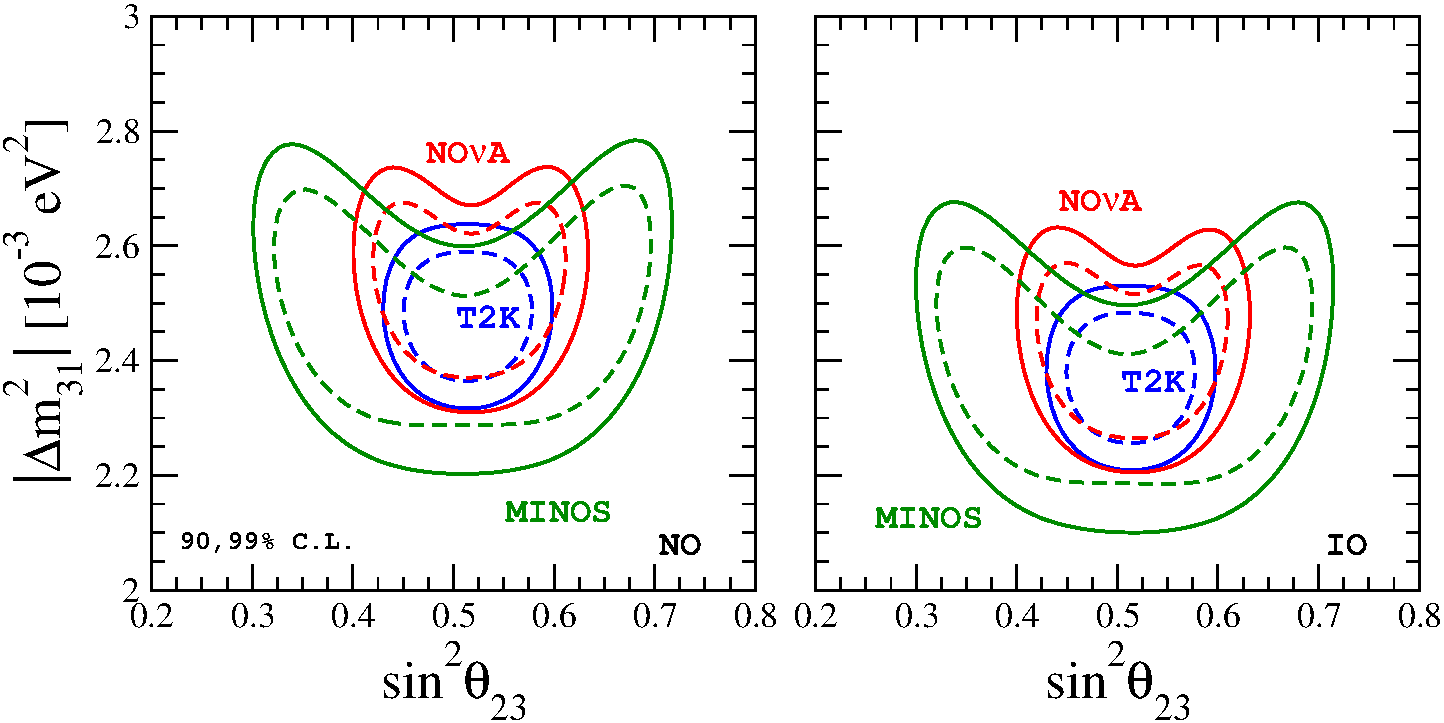
\includegraphics[scale=0.5]{LBL-exp.pdf}
		\caption{90 and 99\% C.L. allowed regions at the $\sin^{2}{\theta_{23}}$-$\Delta{m^{2}_{31}}$ plane for NO (left) and IO (right) as restricted from the long–baseline experiments. Figures adapted from \cite{salas2018}.}
		\label{fig:LBL-exp}
		\end{center}
	\end{figure}

\subsection{Reactor neutrino experiments and $\sin^{2}{2\theta_{13}}$}
	
    Nuclear reactors are prolific sources of $\bar{\nu}_{e}$ with energy near 4 MeV. The oscillation probability can be expressed as
    \begin{gather}
    	P(\bar{\nu}_{e} \rightarrow \bar{\nu}_{e}) = 1-\cos^{4}{\theta_{13}} \sin^{2}{2\theta_{12}} \sin^{2}{\Delta{m^{2}_{21} L/4E}}\notag \\
        -\cos^{2}{\theta_{12}} \sin^{2}{2\theta_{13}} \sin^{2}{\Delta{m^{2}_{31} L/4E}}\notag \\
        -\sin^{2}{\theta_{12}} \sin^{2}{2\theta_{13}} \sin^{2}{\Delta{m^{2}_{32} L/4E}}
    \end{gather}
    
    For short-baseline reactor experiment $L<5$ km we can impose the approximation $\Delta{m^{2}_{32}} \simeq \Delta{m^{2}_{31}}$. The oscillation probability now has the familiar 2-neutrino form with $\theta_{13}$ and $\Delta{m^{2}_{32}}$
    \begin{gather}
    	P(\bar{\nu}_{e} \rightarrow \bar{\nu}_{e}) = 1-\sin^{2}{2\theta_{13}} \sin^{2}{\Delta{m^{2}_{32} L/4E}}
    \end{gather}
    
    The Daya Bay reactor experiment \cite{dayabay} in China release their latest data reporting the detection of more than 2.5 millions of reactor antineutrino events, after 1230 days of taking data \cite{dayabaydata}. This enormous sample together with a significant reduction of systematical errors gives the most precise determination of the reactor mixing angle to date\\
    
    $\sin^{2}{2\theta_{13}} = 0.0841 \pm 0.0027$ (stat.) $\pm 0.0019$ (syst.)\\
    
    The RENO experiment \cite{reno} in South Korea recently reported their data of 500-day observation of the reactor neutrino spectrum \cite{renodata}. Their result is consistent with that of the Daya Bay collaboration\\
    
    $\sin^{2}{2\theta_{13}} = 0.082 \pm 0.009$ (stat.) $\pm 0.006$ (syst.)\\
    
    The latest results from the Double Chooz experiment in France consist of a period of 818 days of data at the far detector and 258 days of data at the near detector. Their best fit result is \cite{doublechoozdata}\\
    
    $\sin^{2}{2\theta_{13}} = 0.119 \pm 0.016$ (stat.$+$syst.)\\
    
    Figure~\ref{fig:sq13-mq31-reactor} shows the 90\% and 99\% C.L. allowed region in the neutrino oscillation parameters $\sin^{2}{\theta_{13}}$ and $\Delta{m^{2}_{31}}$ according to the Daya Bay, RENO, and Double Chooz data for both mass orderings.
    
    \begin{figure}[!hbt]
		\begin{center}
        \centering
        \captionsetup{justification=centering}
		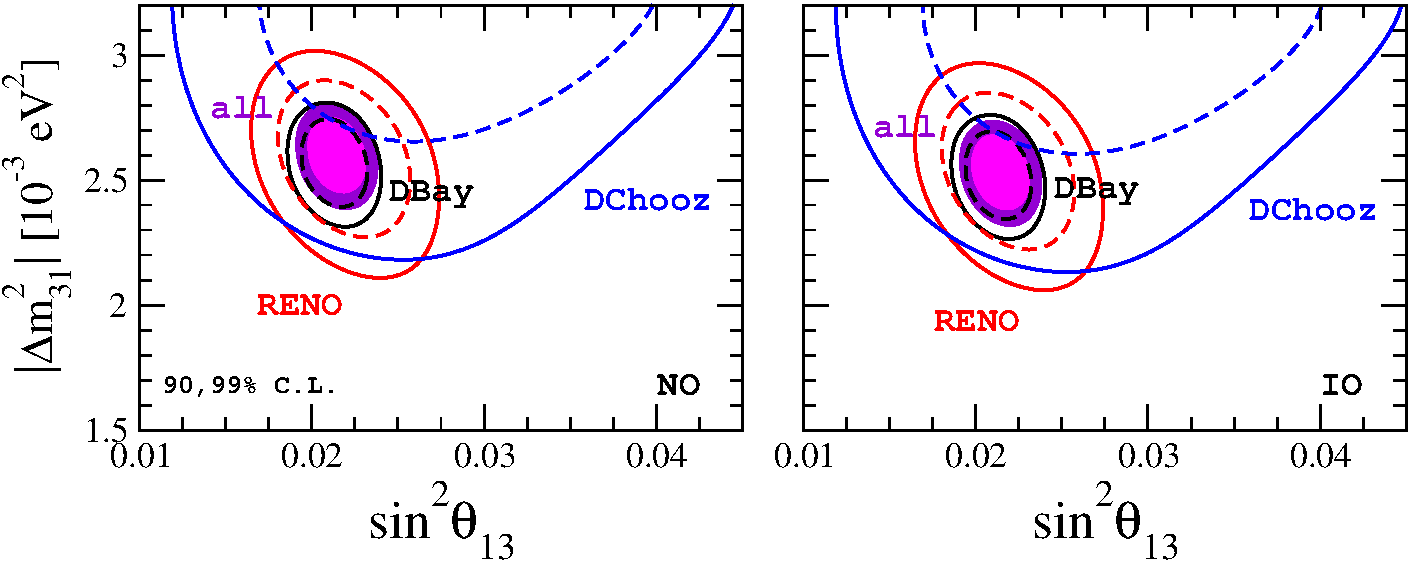
\includegraphics[scale=0.5]{sq13-mq31-reactor.pdf}
		\caption{90 and 99\% C.L. allowed regions at the $\sin^{2}{\theta_{13}}$-$\Delta{m^{2}_{31}}$ plane for NO (left) and IO (right) as restricted from the reactor experiments Daya Bay (black), RENO (red), Double Chooz (blue), and global analysis (coloured regions). Figures adapted from \cite{salas2018}.}
		\label{fig:sq13-mq31-reactor}
		\end{center}
	\end{figure}

\subsection{Solar neutrino sector and $\sin^{2}{\theta_{12}}$, $\Delta{m^{2}_{21}}$}
	
    Solar neutrino experiments are sensitive to $\nu_{e}$ disappearance and have allowed the measurement of $\theta_{12}$ and $\Delta{m^{2}_{21}}$. Solar neutrino analysis includes the historical experiments Homestake \cite{davis1968}, Gallex/GNO \cite{gallex1999}, SAGE \cite{sage1991}, and the more recent, real-time detection experiment Kamiokande \cite{kamiokande}, that confirmed the solar neutrino deficit observed by the previous experiments. Its successor Super-Kamiokande \cite{superk}, with a volume 10 times larger, has provided very precise observations in almost 20 years of operation.
    
    During its fourth, and also last phase, Super-Kamiokande has produced a $3\sigma$ indication of Earth matter effects in the solar neutrino flux by its measure of the day-night asymmetry \cite{superk2016} \cite{superk2016-2} \\
    
    $A_{DN} = \frac{\Phi_{D}-\Phi_{N}}{(\Phi_{D}+\Phi_{N})/2} = (-3.3\pm 1.0$ (stat.)$\pm 0.5$ (syst.)$)$ \% \\ \\
    They have also managed to reconstruct a neutrino survival probability consistent with the MSW prediction at $1\sigma$ \cite{oscmatter} \cite{oscmatter2}.
    
    KamLAND is a reactor neutrino experiment, in which neutrinos are observed through the inverse beta decay process described earlier. The most recent data sample released by KamLAND contains a total live time of 2135 days \cite{kamlanddata}. 
    
    Figure~\ref{fig:sol-sector-sq12-mq21} shows the 90\% and 99\% C.L. allowed region in the parameters $\sin^{2}{\theta_{12}}$ and $\Delta{m^{2}_{21}}$ from the analysis of all solar neutrino data (black lines), from KamLAND data alone (blue lines), and from the combined of both (coloured regions). The best fit result for the global analysis is\\
    
    $\sin^{2}{\theta_{12}} = 0.321^{+0.018}_{-0.016}$ (stat.$+$syst.), 
    $\Delta{m_{21}^{2}} = 7.56\pm 0.19 \times 10^{-5} eV^{2}$\\
    
    \begin{figure}[!hbt]
		\begin{center}
        \centering
        \captionsetup{justification=centering}
		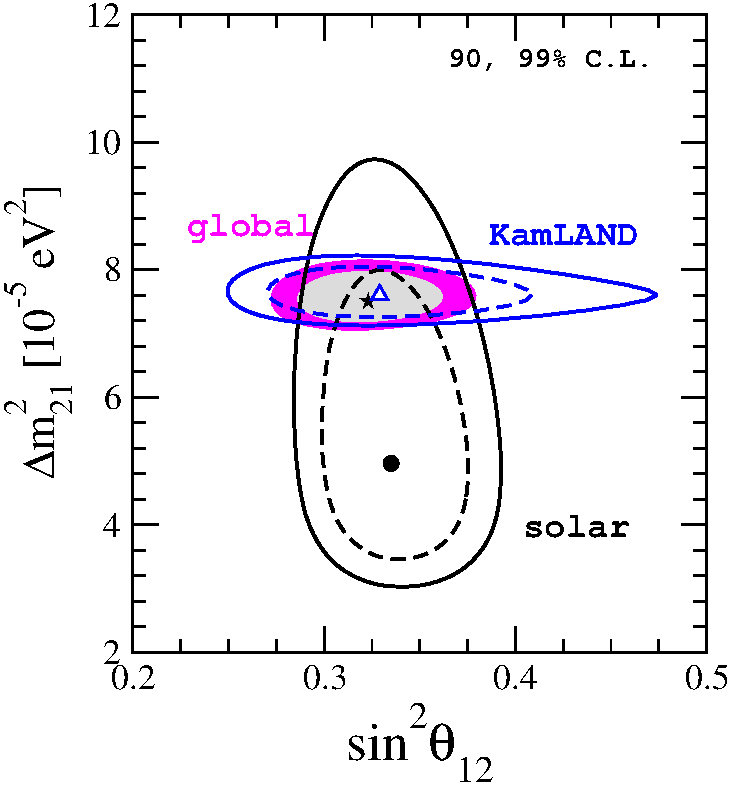
\includegraphics[scale=0.5]{sol-sector-sq12-mq21.pdf}
		\caption{90 and 99\% C.L. allowed regions at the $\sin^{2}{\theta_{13}}$-$\Delta{m^{2}_{31}}$ plane from the analysis of solar neutrino data (black), KamLAND data (blue), and global analysis (coloured regions). Figures adapted from \cite{salas2018}.}
		\label{fig:sol-sector-sq12-mq21}
		\end{center}
	\end{figure}

\subsection{Atmospheric neutrino sector and $\sin^{2}{\theta_{23}}$, $\Delta{m^{2}_{31}}$}
	
    The solution to the previously mentioned Atmospheric Neutrino Anomaly arrived in 1998 when the Super-Kamiokande experiment published their observation of the zenith angle dependence of the $\mu$-like atmospheric neutrino data, suggesting an evidence for neutrino oscillations \cite{superk}. Super-Kamiokande is sensitive to the atmospheric neutrino flux in the range from 100 MeV to TeV. From the latest data sample of Super-Kamiokande atmospheric data, the best fit values for the following oscillation parameters are \cite{superk2017} \\
    
    $\sin^{2}{\theta_{23}} = 0.587$, 
    $\Delta{m_{32}^{2}} = 2.5 \times 10^{-3} eV^{2}$\\
    
    In recent years, atmospheric neutrinos are also being studied by neutrino telescope experiments. IceCube and ANTARES, whose original purpose was to detect higher energy neutrino fluxes, have lowered their energy threshold so that they can measure the most energetic part of the atmospheric neutrino flux. The obtained best fits for the atmospheric oscillation parameters obtained from IceCube most recent data of three-year live time \cite{icecube2015} are\\
    
    $\sin^{2}{\theta_{23}} = 0.53^{+0.09}_{-0.012}$ (stat.$+$syst.),  
    $\Delta{m_{32}^{2}} = 2.72^{+0.19}_{-0.20}\times 10^{-3} eV^{2}$ (stat.$+$syst.)\\
    
    Figure~\ref{fig:atmos-exp} shows the 90\% and 99\% C.L. allowed region in the atmospheric oscillation parameters $\sin^{2}{\theta_{23}}$ and $\Delta{m^{2}_{31}}$ from IceCube DeepCore detector, ANTARES, and Super-Kamiokande phase I to III for both mass orderings.
    
    \begin{figure}[!hbt]
		\begin{center}
        \centering
        \captionsetup{justification=centering}
		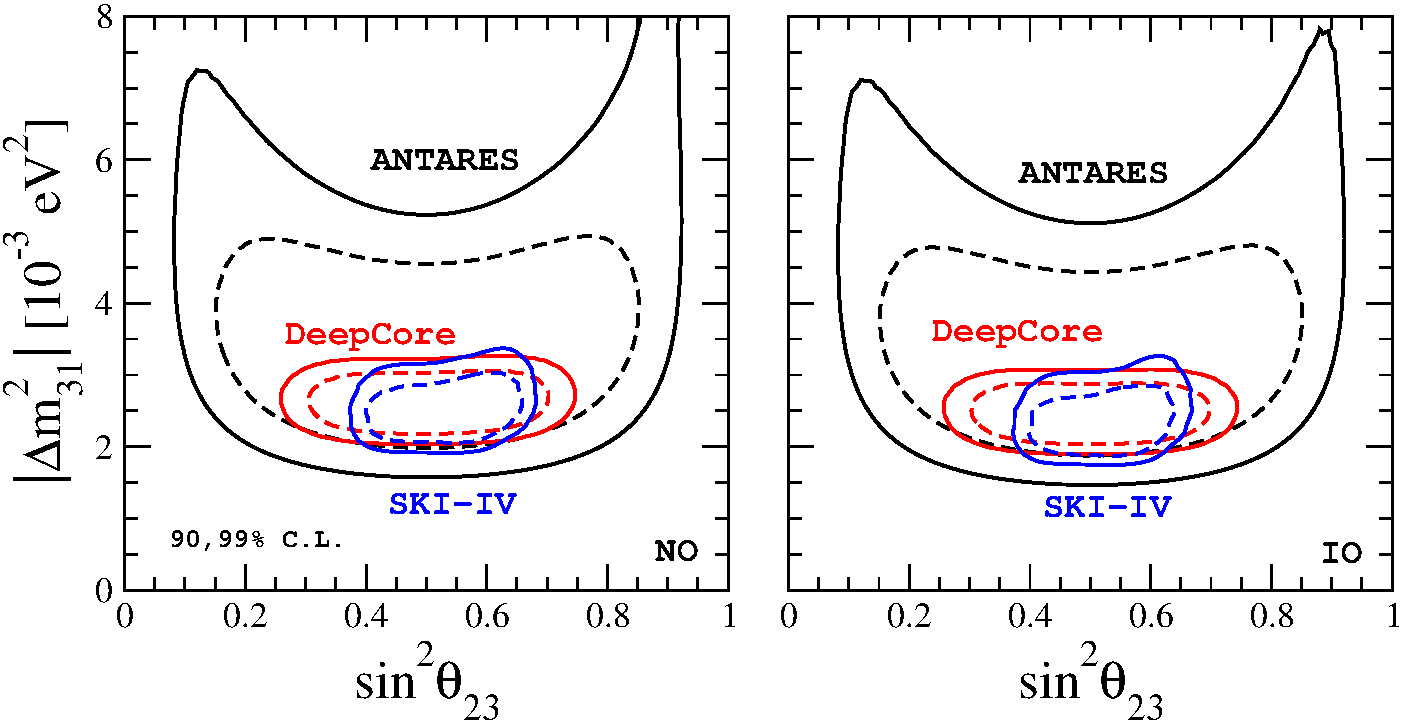
\includegraphics[scale=0.5]{atmos-exp.pdf}
		\caption{90 and 99\% C.L. allowed regions at the $\sin^{2}{\theta_{23}}$-$\Delta{m^{2}_{31}}$ plane for NO (left) and IO (right) as derived from IceCube DeepCore (red), ANTARES (black), and Super-Kamiokande phase I-III (blue). Figures adapted from \cite{salas2018}.}
		\label{fig:atmos-exp}
		\end{center}
	\end{figure}

\subsection{Global fit and Comments}
	
    The main aim of global analyses of neutrino oscillation data is that although different experiments are heavily sensitive to only one or two oscillation parameters, in combination with the rest of data samples relevant information on the neutrino oscillation parameters can be discovered. Table~\ref{global-fit} shows the results of a global analysis of the data within the standard 3-neutrino mixing framework.
    
    Figure~\ref{fig:fullfit} summarises the latest global fit adapted from \cite{salas2018}. Despite the remarkable sensitivity reached in the determination of most of the neutrino oscillation parameters, there are still three unknown parameters in the standard 3-neutrino mixing scheme: the octant of $\theta_{23}$, the value of the CP phase $\delta$ and the neutrino mass ordering.
    
    \begin{figure}[!hbt]
		\begin{center}
        \centering
		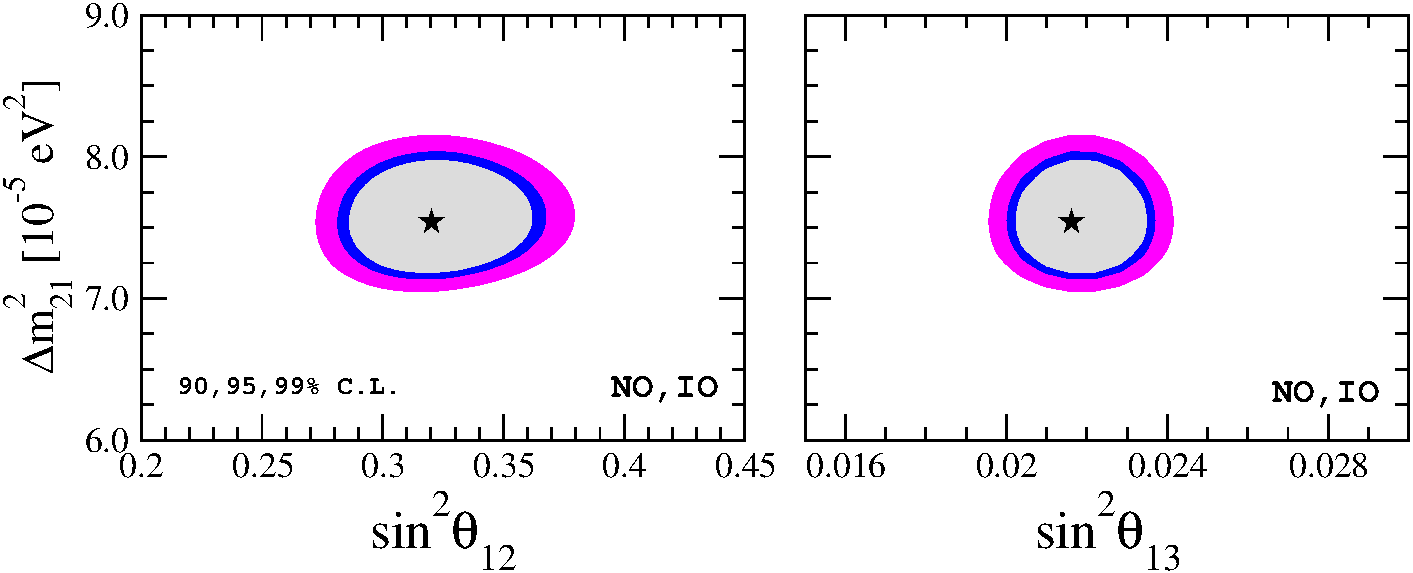
\includegraphics[scale=0.4]{sq12-sq13-mq21.pdf}
		\end{center}
	\end{figure}
    \begin{figure}[!hbt]
		\begin{center}
        \centering
		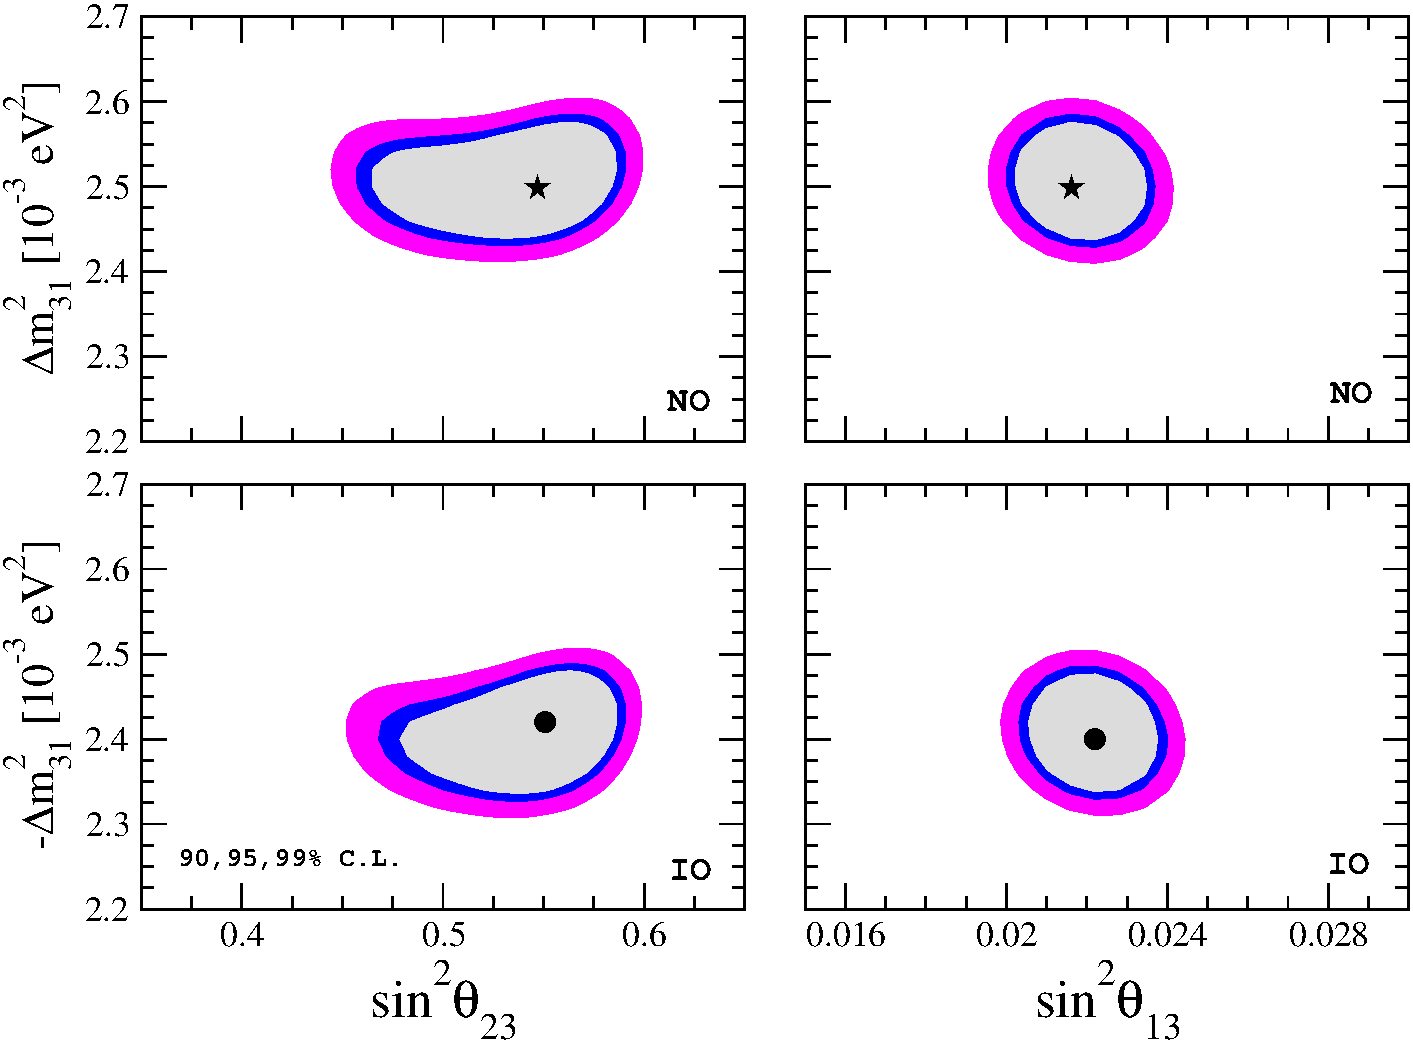
\includegraphics[scale=0.4]{sq23-sq13-mq31.pdf}
		\end{center}
	\end{figure}
    \begin{figure}[!hbt]
		\begin{center}
        \centering
        \captionsetup{justification=centering}
		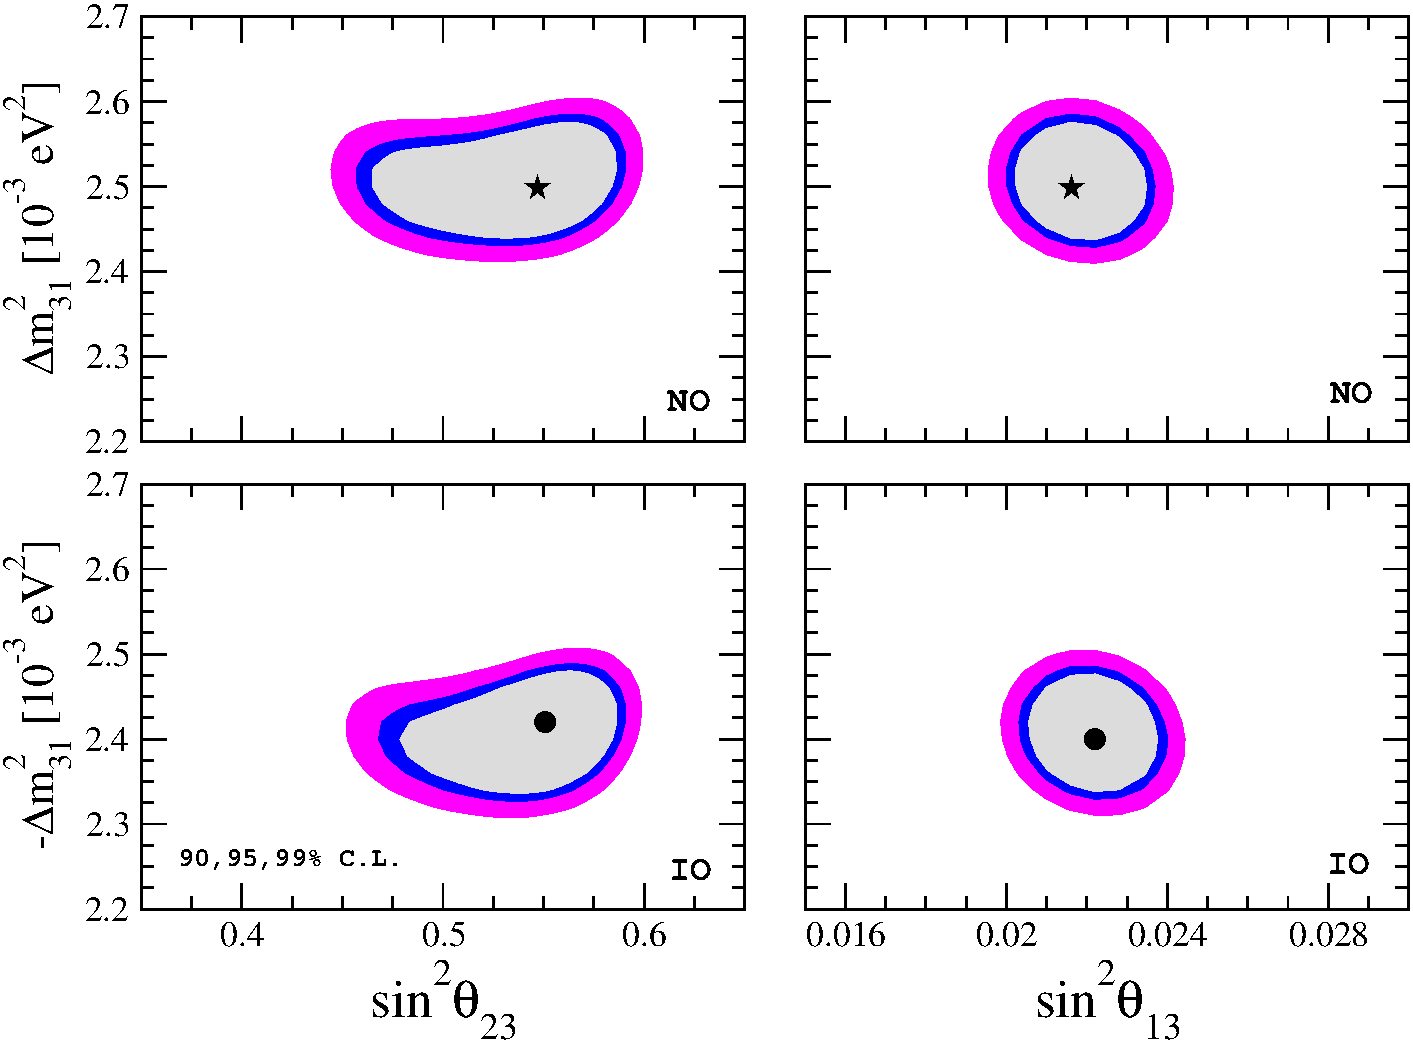
\includegraphics[scale=0.4]{sq23-sq13-mq31.pdf}
        \caption{Global fit summary 2018 for both mass ordering schemes. Regions correspond to 90, 95, and 99\% C.L.. Figures adapted from \cite{salas2018}.}
        \label{fig:fullfit}
		\end{center}
	\end{figure}
    
    \clearpage
    So far, experimental neutrino data have not indicated a conclusive preference for values of $\theta_{23}$ smaller, equal or larger than $\pi /4$. However, this may change after the implementation of the partially published data release of T2K \cite{t2kpartial} in the global fit.
    
    In the same way, we are still not sure which neutrino mass ordering scheme is preferred, and we will have to wait for the next generation of experiments designed for this purpose, such as DUNE \cite{dune}, JUNO \cite{juno}, or RENO-50 \cite{reno50}.
    
    The result also shows that the current global sensitivity to the CP phase is dominated by the T2K experiment, which is due to the release of T2K results from its antineutrino run. The current best fit values for the CP violating phase are located at $\delta=1.21\pi$ for NO and at  $\delta=1.56\pi$ for IO.

	\begin{table}[!hbt]
    \begin{center}
    \centering
    \captionsetup{justification=centering}
  \catcode`?=\active \def?{\hphantom{0}}
   \begin{tabular}{lccc}
    \hline
    parameter & best fit $\pm$ $1\sigma$ &   \hphantom{x} 2$\sigma$ range  \hphantom{x} &  \hphantom{x} 3$\sigma$ range  \hphantom{x}
    \\
    \hline
    $\Delta m^2_{21}\: [10^{-5} eV^{2}]$
    & 7.55$^{+0.20}_{-0.16}$  & 7.20--7.94 & 7.05--8.14 \\[3mm] 
    %%
    $|\Delta m^2_{31}|\: [10^{-3} eV^{2}]$ (NO)
    &  2.50$\pm$0.03 &  2.44--2.57 &  2.41--2.60\\
     $|\Delta m^2_{31}|\: [10^{-3} eV^{2}]$ (IO)
    &  2.42$^{+0.03}_{-0.04}$ &  2.34--2.47 &  2.31-2.51 \\[3mm]
    %%
    $\sin^2\theta_{12} / 10^{-1}$
    & 3.20$^{+0.20}_{-0.16}$ & 2.89--3.59 & 2.73--3.79\\
    $\theta_{12} /^\circ$ & 34.5$^{+1.2}_{-1.0}$ & 32.5--36.8 & 31.5--38.0 \\[3mm]
    %%
     $\sin^2\theta_{23} / 10^{-1}$ (NO)
              &	5.47$^{+0.20}_{-0.30}$ & 4.67--5.83 & 4.45--5.99 \\
     $\theta_{23} /^\circ$ &	47.7$^{+1.2}_{-1.7}$ &  43.1--49.8& 41.8--50.7\\ 
     $\sin^2\theta_{23} / 10^{-1}$ (IO)
              & 5.51$^{+0.18}_{-0.30}$ & 4.91--5.84 & 4.53--5.98\\
     $\theta_{23} /^\circ$ & 47.9$^{+1.0}_{-1.7}$ & 44.5--48.9 & 42.3--50.7\\[3mm] 
    %%
    $\sin^2\theta_{13} / 10^{-2}$ (NO)
    & 2.160$^{+0.083}_{-0.069}$ &  2.03--2.34 & 1.96--2.41 \\
    $\theta_{13} /^\circ$    & 8.45$^{+0.16}_{-0.14}$ & 8.2--8.8 & 8.0--8.9 \\
    $\sin^2\theta_{13} / 10^{-2}$ (IO)
    & 2.220$^{+0.074}_{-0.076}$ & 2.07--2.36 & 1.99--2.44 \\
    $\theta_{13} /^\circ$ & 8.53$^{+0.14}_{-0.15}$ & 8.3--8.8 &  8.1--9.0 \\[3mm]
    %%
   $\delta/\pi$ (NO)
   	& 1.21$^{+0.21}_{-0.15}$ & 1.01--1.75 & 0.87--1.94 \\
   $\delta/^\circ$	& 218$^{+38}_{-27}$ & 182--315 & 157--349\\
    $\delta/\pi$ (IO)
   	& 1.56$^{+0.13}_{-0.15}$ & 1.27--1.82 & 1.12--1.94 \\
   $\delta/^\circ$	& 281$^{+23}_{-27}$ & 229--328 & 202--349\\
       \hline
     \end{tabular}
     \caption{ \label{tab:sum-2018}
        Neutrino oscillation parameters summary determined from the global analysis in \cite{salas2018}. The ranges for inverted ordering refer to the local minimum for this neutrino mass ordering.
     }
     \label{global-fit}
    \end{center}
	\end{table}

\clearpage    
\begin{thebibliography}{99}

	\bibitem{pauliletter1930}
    Pauli W., 1930. "Open letter to the group of radioactive people at the Gauverein meeting in T\"{u}bingen". \textit{Pauli Archive at CERN}.
    \bibitem{fermi1934}
    Fermi E., 1934. "Tentativo Di Una Teoria Dei Raggi $\beta$". \textit{Nuovo Cim.}, 11, 1.
    \bibitem{bethepeierls1934}
    Bethe H., Peierls R., 1934. \textit{Nature}, 133, 532.
    \bibitem{cowanreines1956}
    Cowan C. L. \textit{et al.}, 1956. "Detection of the Free Neutrino: a Confirmation". \textit{Science}, 124, 103.
    \bibitem{wu1957}
    Wu C. S. \textit{et al.}, 1957. "Experimental Test of Parity Conservation in Beta Decay". \textit{Phys. Rev.}, 105, 1413.
    \bibitem{salam1956}
    Salam A., 1957. "On Parity Conservation and Neutrino Mass". \textit{Nuovo Cim.}, 5, 299.
    \bibitem{landau1957}
    Landau L., 1957. "On the Conservation Laws for Weak Interactions". \textit{Nucl. Phys.}, 3, 127.
    \bibitem{leeyang1957}
    Lee. T. D., Yang C. N., 1957. "Parity Nonconservation and a Two-Component Theory of the Neutrino". \textit{Phys. Rev.}, 105, 1671.
    \bibitem{weyl1929}
    Weyl H., 1929. "Elektron und Gravitation. I.". \textit{Z. Physik}, 56, 330.
    \bibitem{garwinledermanweinrich1957}
    Garwin R. L., Lederman L. M., Weinrich M., 1957. "Observations of the Failure of Conservation of Parity and Charge Conjugation in Meson Decays: the Magnetic Moment of the Free Muon". \textit{Phys. Rev.}, 105, 1415.
    \bibitem{goldhabergrodzinssunyar1958}
    Goldhaber M., Grodzins L., Sunyar A. W., 1958. "Helicity of Neutrinos". \textit{Phys. Rev.}, 109, 1015.
    \bibitem{feynmangellmann1958}
    Feynman R. P., Gell-Mann M., 1958. "Theory of the Fermi Interaction". \textit{Phys. Rev.}, 109, 193.
    \bibitem{sudarshanmarshak1958}
    Sudarshan E. C. G., Marshak R. E., 1958. "Chirality Invariance and the Universal Fermi Interaction". \textit{Phys. Rev.}, 109, 1860.
    \bibitem{glashow1961}
    Glashow S. L., 1961. "Partial-symmetries of Weak Interactions". \textit{Nucl. Phys.}, 22, 579.
    \bibitem{goldstonesalamweinberg1962}
    Goldstone J., Salam A., Weinberg S., 1962. "Broken Symmetries". \textit{Phys. Rev.}, 127, 965.
    \bibitem{weinberg1967}
    Weinberg S., 1967. "A Model of Leptons". \textit{Phys. Rev. Lett.}, 19, 1264.
    \bibitem{grosswilczek1973}
    Gross D. J., Wilczek F., 1973. "Ultraviolet Behavior of Non-Abelian Gauge Theories". \textit{Phys. Rev. Lett.}, 30, 1343.
    \bibitem{politzer1973}
    Politzer H. D., 1973. "Reliable Pertubative Results for Strong Interactions?". \textit{Phys. Rev. Lett.}, 30, 1346.
    \bibitem{davis1968}
    Davis R., Harmer D. S., Hoffman K. C., 1968. "Search for Neutrinos from the Sun". \textit{Phys. Rev. Lett.}, 20, 1205.
    \bibitem{davis1998}
    Cleveland B. T. \textit{et al.}, 1998. "Measurement of the Solar Electron Neutrino Flux with the Homestake Chlorine Detector". \textit{The Astrophys. Jour.}, 496, 505.
    \bibitem{bahcall2004}
    Bahcall J. N., Pinsonneault M. H., 2004. "What Do We (Not) Know Theoretically about Solar Neutrino Fluxes?". \textit{Phys. Rev. Lett.}, 92, 121301.
    \bibitem{kamiokande1991}
    \textit{Kamiokande Collaboration}, 1991. "Real-time, directional measurement of ${}^{8} B$ solar neutrinos in the Kamiokande II detector". \textit{Phys. Rev.}, D44, 2241.
    \bibitem{superk2016}
    \textit{Super-Kamiokande Collaboration}, 2016. "Solar Neutrino Measurements in Super-Kamiokande-IV". \textit{Phys. Rev.}, D94, 052010.
    \bibitem{sage1991}
    \textit{SAGE Collaboration}, 1991. "Search for Neutrinos from the Sun Using the Reaction ${}^{71}$Ga($\nu_{e}$,$e^{-}$)${}^{71}$Ge". \textit{Phys. Rev. Lett.}, 67, 3332.
    \bibitem{gallex1999}
    \textit{GALLEX Collaboration}, 1999. "GALLEX solar neutrino observations: results for GALLEX IV". \textit{Phys. Lett.}, B447, 127.
    \bibitem{sno2001}
    \textit{SNO Collaboration}, 2001. "Measurement of the Rate of $\nu_{e} +d \rightarrow p+p+e^{-}$ Interactions Produced by ${}^{8}$B Solar Neutrinos at the Sudbury Neutrino Observatory". \textit{Phys. Rev. Lett.}, 87, 071301.
    \bibitem{hirata1998}
    Hirata K. S. \textit{et al.}, 1988. "Experimental Study of the Atmospheric Neutrino Flux". \textit{Phys. Lett.}, B205, 416.
    \bibitem{casper1991}
    Casper D. \textit{et al.}, 1991. "Measurement of Atmospheric Neutrino Composition with the IMB-3 Detector". \textit{Phys. Rev. Lett.}, 66, 2561.
    \bibitem{macro1998}
    \textit{MACRO Collaboration}, 1998. "Measurement of the Atmospheric Neutrino-induced Upgoing Muon Flux Using MACRO". \textit{Phys. Lett}, B434, 451.
    \bibitem{pontecorvo1957}
    Pontecorvo B., 1957. "Mesonium and Antimesonium". \textit{JETP}, 6, 429.
    \bibitem{gellmann1955}
    Gell-Mann M., Pais A., 1955. "Behavior of Neutral Particles under Charge Conjugation". \textit{Phys. Rev.}, 97, 1387.
    \bibitem{mns1962}
    Maki Z. Nakagawa M., Sakata S., 1962. "Remarks on the Unified Model of Elementary Particles". \textit{Prog. of Theo. Phys.}, 28, 870.
    \bibitem{pontecorvo1967}
    Pontecorvo B., 1967. "Neutrino Experiments and the Problem of Conservation of Leptonic". \textit{JETP}, 26, 984.
    \bibitem{pontecorvo1969}
    Gribov V., Pontecorvo B., 1969. "Neutrino Astronomy and Lepton Charge". \textit{Phys. Lett.}, 28B, 493.
    \bibitem{fulltheory70s}
    Bilenky S. M., Pontecorvo B., 1976. \textit{Phys. Lett.} B61, 248.\\
    Bilenky S. M., Pontecorvo B., 1976. \textit{Lett. Nuovo Cim.} 17, 569.\\ 
    Bilenky S. M., Pontecorvo B., 1978. \textit{Phys. Rep.} 41, 225.\\
    Eliezer S., Swift A., 1976. \textit{Nucl. Phys.} B105, 45.\\
    Fritzsch H., Minkowski P., 1976. \textit{Phys. Lett.} B62, 72.
    \bibitem{esteban2017}
    Esteban I., Gonzalez-Garcia M. C., Maltoni M., Martinez-Soler I., Schwetz T., 2017. "Updated fit to three neutrino mixing: exploring the accelerator-reactor complementarity". \textit{JHEP}, 1, 87.
    \bibitem{capozzi2017}
    Capozzi F., Valentino E. D., Lisi E., Marrone A., Melchiorri A., Palazzo A., 2017. "Global constraints on absolute neutrino masses and their ordering". \textit{Phys. Rev.}, D95, 096014.
    \bibitem{salas2018}
    de Salas. P. F., Forero D. V., Ternes C. A., Tórtola M., Valle J. W. F., 2018. "Status of neutrino oscillations 2018: first hint for normal mass ordering and improved CP sensitivity". arXiv:1708.01186v2.
    \bibitem{k2k}
    \textit{K2K Collaboration}, 2006. "Measurement of Neutrino Oscillation by the K2K Experiment". \textit{Phys. Rev.}, D74, 072003.
    \bibitem{minos}
    \textit{MINOS Collaboration}, 1998. "The MINOS Detectors Technical Design Report".
    \bibitem{opera}
     Acquafredda R. \textit{et al}, 2009. "The OPERA experiment in the CERN to Gran Sasso neutrino beam". \textit{JINST} 4, 04018.
    \bibitem{icarus}
    \textit{ICARUS Collaboration}, 2001. "The ICARUS experiment, a second-generation proton decay experiment and neutrino observatory at the Gran Sasso Laboratory". arXiv:hep-ex/0103008.
    \bibitem{kamiokande}
    \textit{Kamiokande-II Collaboration}, 1988. "Experimental Study of the Atmospheric Neutrino Flux". \textit{Phys. Lett.}, B205, 416.
    \bibitem{imb}
    Haines T. \textit{et al.}, 1986. "Calculation of Atmospheric Neutrino Induced Backgrounds in a Nucleon Decay Search". \textit{Phys. Rev. Lett.} 57, 1986.
    \bibitem{superk}
    \textit{Super-Kamiokande Collaboration}, 1998. "Evidence for oscillation of atmospheric neutrinos". \textit{Phys. Rev. Lett.}, 81, 1562.
    \bibitem{chooz}
     \textit{CHOOZ Collaboration}, 2003. "Search for neutrino oscillations on a long baseline at the CHOOZ nuclear power station". \textit{Eur. Phys. Jour.}, C27, 331.
    \bibitem{t2k}
    \textit{T2K Collaboration}, 2011. "The T2K Experiment". \textit{Nucl. Instrum. Meth.}, A659, 106.
    \bibitem{nova}
    \textit{NO$\nu$A Collaboration}, 2007. "The NO$\nu$A Technical Design Report". \textit{FERMILAB-DESIGN-2007-01}.
    \bibitem{minosdata}
    \textit{MINOS Collaboration}, 2014. "Combined analysis of $\nu_{\mu}$ disappearance and $\nu_{\mu} \rightarrow \nu_{e}$ appearance in MINOS using
accelerator and atmospheric neutrinos". \textit{Phys. Rev. Lett.}, 112, 191801.
	\bibitem{t2kdata}
    \textit{T2K Collaboration}, 2017. "Combined Analysis of Neutrino and Antineutrino Oscillations at T2K". \textit{Phys. Rev. Lett.}, 118, 151801.
    \bibitem{dayabay}
    \textit{Daya Bay Collaboration}, 2012. "Observation of electron-antineutrino disappearance at Daya Bay". \textit{Phys. Rev. Lett.} 108, 171803.
    \bibitem{dayabaydata}
    \textit{Daya Bay Collaboration}, 2016. "Measurement of electron antineutrino oscillation based on 1230 days of operation of the Daya Bay experiment". arXiv: 1610.04802.
    \bibitem{reno}
    \textit{RENO Collaboration}, 2012. "Observation of Reactor Electron Antineutrino Disappearance in the RENO Experiment". \textit{Phys. Rev. Lett.}, 108, 191802.
    \bibitem{renodata}
    \textit{RENO Collaboration}, 2017. "Spectral Measurement of the Electron Antineutrino Oscillation Amplitude and Frequency using 500 Live Days of RENO Data". arXiv:1610.04326.
    \bibitem{doublechoozdata}
    \textit{Double Chooz Collaboration}, 2017. "Multi-detector results from the Double Chooz experiment". \textit{Double Chooz Publication}.
    \bibitem{superk2016-2}
    \textit{Super-Kamiokande Collaboration}, 2016. "Solar neutrino results from Super-Kamiokande". \textit{Super-Kamiokande Publication}.
    \bibitem{oscmatter}
    Wolfenstein L., 1978. "Neutrino Oscillations in Matter". \textit{Phys. Rev.}, D17, 2369.
    \bibitem{oscmatter2}
    Mikheev S. P., Smirnov A. Y., 1985. "Resonance Amplication of Oscillations in Matter and Spectroscopy of Solar Neutrinos". \textit{Sov. Jour. Nucl. Phys.}, 42, 913.
    \bibitem{kamlanddata}
    \textit{KamLAND Collaboration}, 2011. "Constraints on $\theta_{13}$ from A Three-Flavor Oscillation Analysis of Reactor Antineutrinos at KamLAND". \textit{Phys. Rev.}, D83, 052002.
    \bibitem{superk2017}
    \textit{Super-Kamiokande Collaboration}, 2017. "Solar and atmospheric neutrino oscillations in Super-Kamiokande," \textit{PoS NOW 2016}, 001.
    \bibitem{icecube2015}
    \textit{IceCube Collaboration}, 2015. "Determining neutrino oscillation parameters from atmospheric muon neutrino disappearance with three years of IceCube DeepCore data". \textit{Phys. Rev.}, D91, 072004.
    \bibitem{t2kpartial}
    \textit{T2K Collaboration}, 2017. "T2K Neutrino Oscillation Results with Data Up To 2017 Summer". \textit{T2K Publication}.
    \bibitem{dune}
    \textit{DUNE Collaboration}, 2016. "Long-Baseline Neutrino Facility (LBNF) and Deep Underground Neutrino Experiment (DUNE)". arXiv:1512.06148.
    \bibitem{juno}
    \textit{JUNO Collaboration}, 2016. "Neutrino Physics with JUNO". \textit{Jour. Phys.}, G43, 030401.
    \bibitem{reno50}
    Kim S.B. 2015. "New results from RENO and prospects with RENO-50". \textit{Nucl. Part. Phys. Proc.}, 265, 93.
    
\end{thebibliography}



\end{document}